\documentclass[tikz,border=3mm]{standalone}
\usetikzlibrary{angles,quotes}
\tikzset{
    myangle/.style={
        draw,
        angle radius=6mm,
        angle eccentricity=1.7,
        }
}

\begin{document}
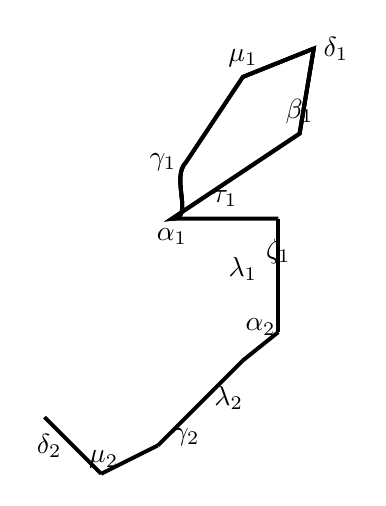
\begin{tikzpicture}[scale=1.8]
    \coordinate[label=above:$\mu_1$] (M1) at (-0.5,2);
    \coordinate[label=right:$\delta_1$] (D1) at (0,2.2);
    \coordinate[label=left:$\gamma_1$] (G1) at (-0.9,1.4);
    \coordinate[label=below:$\alpha_1$] (A1) at (-1,1);
    \coordinate[label=above:$\beta_1$] (B1) at (-0.1,1.6);
    \draw[line width=0.5mm] (A1) to[out=0,in=-135] (G1)
                             -- (M1) -- (D1) -- (B1) -- cycle;
    \coordinate[label=below:$\lambda_1$] (L1) at (-0.5,0.8);
    \draw[line width=0.5mm] (A1) to[out=0,in=-135] (G1)
                             -- (M1) -- (D1) -- (B1) -- cycle;
    \draw[line width=0.5mm] (A1) to[out=0,in=-135] (G1);
    \draw[line width=0.5mm] (M1) -- (D1);
    \draw[line width=0.5mm] (B1) -- (D1);

    % Gap between $\beta_1$ and $\alpha_2$ caused by $\tau_1$ and $\zeta_1$
    \draw[line width=0.5mm] (A1) -- node[above=0.2] {$\tau_1$} (-0.25,1);
    \draw[line width=0.5mm] (-0.25,1) -- node[above] {$\zeta_1$} (-0.25,0.2);
    \draw[line width=0.5mm] (-0.25,0.2) -- node[above] {$\alpha_2$} (-0.5,0);
    \draw[line width=0.5mm] (-0.5,0) -- node[below] {$\lambda_2$} (-0.7,-0.2);
    \draw[line width=0.5mm] (-0.7,-0.2) -- node[below] {$\gamma_2$} (-1.1,-0.6);
    \draw[line width=0.5mm] (-1.1,-0.6) -- node[left] {$\mu_2$} (-1.5,-0.8);
    \draw[line width=0.5mm] (-1.5,-0.8) -- node[left] {$\delta_2$} (-1.9,-0.4);
\end{tikzpicture}
\end{document}